\section{Testing procedures} \label{sec:test}

The purpose of this testing procedure is to verify that the custom board you have received is fully functional. They have all been already tested once but this is a good occasion for you to get your hands into the hardware for the first time! If you have any issue later on, start by re-doing this procedure and if it does not work, contact us to start the debugging together.

\subsection{Basic functionalities}

Please make sure you carry out this procedure the first time you get your boards.

\begin{itemize}
    \item Set the boards in \textit{Development mode}, see Section \ref{sec:mode-dev}.
    \item Make sure the "PWR LED" is ON.
    \item Make sure the AFE part is supplied (by connecting jumpers SUP+ and SUP-).
    \item Connect an oscilloscope to monitor the 3V3\_MAIN signal and the SOUND signal.
    \item Connect your PC audio through the mini-jack input on the board.
    \item Use a jumper to connect SEL\_SOUND to 1 (JACK): you should see the signal clearly on the oscilloscope (make sure the sound level on your computer is high enough). The signal should be centered around 1.65 V.
    \item Finally, move the jumper to connect SEL\_SOUND to 3 (AFE). Clap in your hands or say something: you should see it clearly on the oscilloscope (1V scale). The signal should be centered around 1.65 V.
    \item If you got here without any issue, the basic functionalities of the power-management board are working properly. Note that the EH part of the power-management board is not covered here.
\end{itemize}


\subsection{EH circuit only}

\begin{itemize}
    \item Set the boards as presented in Fig. \ref{fig:testing-mode-eh}.
    \item Connect an oscilloscope to monitor the signals highlighted with a purple star in Fig. \ref{fig:testing-mode-eh}. Nothing should happen if no PV cell is connected.
    \item Then, connect one PV cell (and double-check the polarity!). You can connect two PV cells but it is not necessary.
    \item You should see the BATT signal rising as energy is harvested from the environment thanks to the harvesting circuit and stored in the capacitor (C = 1 mF). When the BATT signal reaches a specific value (check out the AEM10941 datasheet!), it switches on the EH outputs i.e., 3V3\_EH and 1V8\_EH. Can you see that ?
    \item If the AFE part is supplied (jumpers SUP+ and SUP- connected), it should slowly draw energy from the capacitor.
    \item Make sure that SEL\_SOUND is connected to 3 (AFE). Clap in your hands or say something: you should see it clearly on the oscilloscope. Note: you could also power the AFE with the 3V3\_EH if you want but you need to make sure you connect the right pins: please ask support if you are not 100\% sure how to do it !
    \item If you got here without any issue, it means that the EH part of your power-management board seems to work properly.
\end{itemize}

\begin{figure}[h!]
    \centering
    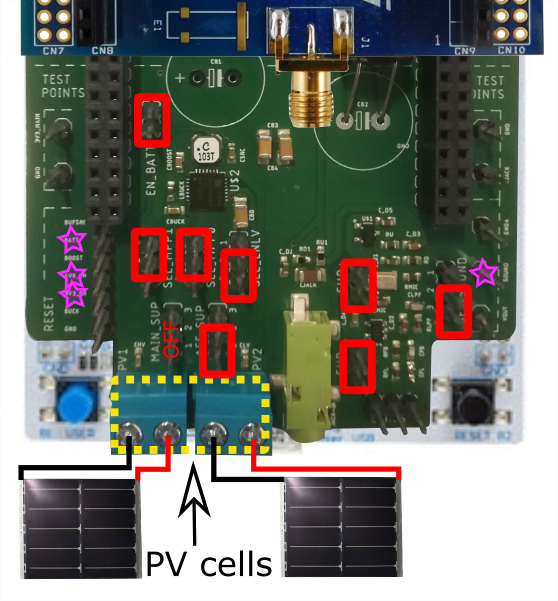
\includegraphics[width=0.5\textwidth]{figs/testing-EH.png}
    \caption{Specific settings for the power management board in order to test the EH circuit. Other jumpers must be set as shown in Fig. \ref{fig:settings-mode-eh}.}
    \label{fig:testing-mode-eh}
\end{figure}

\vspace{0.5cm}
\flushright
That's all folks !
